% !TEX encoding = UTF-8 Unicode
%%%%%%%%%%%%%%%%%%%%%%%%%%%%%%%%%%%%%%%%%
% Beamer Presentation
% LaTeX Template
% Version 1.0 (10/11/12)
%
% This template has been downloaded from:
% http://www.LaTeXTemplates.com
%
% License:
% CC BY-NC-SA 3.0 (http://creativecommons.org/licenses/by-nc-sa/3.0/)
%
%%%%%%%%%%%%%%%%%%%%%%%%%%%%%%%%%%%%%%%%%

%----------------------------------------------------------------------------------------
%	PACKAGES AND THEMES
%----------------------------------------------------------------------------------------

\documentclass{beamer}

\mode<presentation> {

% The Beamer class comes with a number of default slide themes
% which change the colors and layouts of slides. Below this is a list
% of all the themes, uncomment each in turn to see what they look like.

%\usetheme{default}
%\usetheme{AnnArbor}
%\usetheme{Antibes}
%\usetheme{Bergen}
%\usetheme{Berkeley}
%\usetheme{Berlin}
%\usetheme{Boadilla}
%\usetheme{CambridgeUS}
%\usetheme{Copenhagen}
%\usetheme{Darmstadt}
%\usetheme{Dresden}
%\usetheme{Frankfurt}
%\usetheme{Goettingen}
%\usetheme{Hannover}
%\usetheme{Ilmenau}
%\usetheme{JuanLesPins}
%\usetheme{Luebeck}
\usetheme{Madrid}
%\usetheme{Malmoe}
%\usetheme{Marburg}
%\usetheme{Montpellier}
%\usetheme{PaloAlto}
%\usetheme{Pittsburgh}
%\usetheme{Rochester}
%\usetheme{Singapore}
%\usetheme{Szeged}
%\usetheme{Warsaw}

% As well as themes, the Beamer class has a number of color themes
% for any slide theme. Uncomment each of these in turn to see how it
% changes the colors of your current slide theme.

%\usecolortheme{albatross}
%\usecolortheme{beaver}
%\usecolortheme{beetle}
%\usecolortheme{crane}
%\usecolortheme{dolphin}
%\usecolortheme{dove}
%\usecolortheme{fly}
%\usecolortheme{lily}
%\usecolortheme{orchid}
%\usecolortheme{rose}
%\usecolortheme{seagull}
%\usecolortheme{seahorse}
%\usecolortheme{whale}
%\usecolortheme{wolverine}

%\setbeamertemplate{footline} % To remove the footer line in all slides uncomment this line
%\setbeamertemplate{footline}[page number] % To replace the footer line in all slides with a simple slide count uncomment this line

%\setbeamertemplate{navigation symbols}{} % To remove the navigation symbols from the bottom of all slides uncomment this line
}

\usepackage{graphicx} % Allows including images
\usepackage{booktabs} % Allows the use of \toprule, \midrule and \bottomrule in tables
\usepackage{xeCJK}
\setCJKmainfont{SourceHanSerif-Regular}
\usepackage{color}
\usepackage{listings}
\lstset{numbers=left}
\usepackage{tikz}


%----------------------------------------------------------------------------------------
%	TITLE PAGE
%----------------------------------------------------------------------------------------

\title[Sockets]{Sockets} % The short title appears at the bottom of every slide, the full title is only on the title page

\author{张海宁} % Your name
\institute[计算机科学与技术学院] % Your institution as it will appear on the bottom of every slide, may be shorthand to save space
{
贵州大学 \\ % Your institution for the title page
\medskip
\textit{hnzhang1@gzu.edu.cn} % Your email address
}
\date{\today} % Date, can be changed to a custom date

\begin{document}

\begin{frame}
\titlepage % Print the title page as the first slide
\end{frame}

\begin{frame}
\frametitle{Overview} % Table of contents slide, comment this block out to remove it
\tableofcontents % Throughout your presentation, if you choose to use \section{} and \subsection{} commands, these will automatically be printed on this slide as an overview of your presentation
\end{frame}

%----------------------------------------------------------------------------------------
%	PRESENTATION SLIDES
%----------------------------------------------------------------------------------------
\section{Sockets}
\begin{frame}
\Huge{\centerline{Sockets}}
\end{frame}
\subsection{What is a Socket}
\begin{frame}
\Huge{\centerline{What is a Socket}}
\end{frame}
\begin{frame}{Socket}
Socket是一种进程间的通信机制。
\begin{block}{进程间通信}
\center{
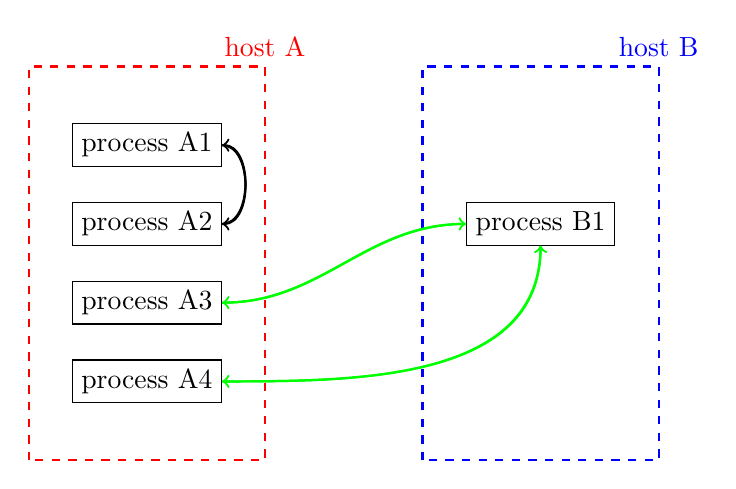
\begin{tikzpicture}
\draw [thick,red,dashed,above] (0,0) rectangle (3,5) node{host A};
\node [draw,rectangle] (pa1) at(1.5,4){process A1};
\node [draw,rectangle] (pa2) at(1.5,3){process A2};
\node [draw,rectangle] (pa3) at(1.5,2){process A3};
\node [draw,rectangle] (pa4) at(1.5,1){process A4};
\draw [thick,blue,dashed,above] (5,0) rectangle (8,5)node{host B};
\node [draw,rectangle] (pb1) at(6.5,3){process B1};
%\node [draw,rectangle] (pb2) at(6.5,2){...};
\draw[thick,->](pa1) to[out=0,in=360] (pa2);
\draw[thick,->](pa2) to[out=0,in=360] (pa1);
\draw[thick,->,green](pa3) to[out=0,in=180] (pb1);
\draw[thick,->,green](pa4) to[out=0,in=270] (pb1);
\draw[thick,->,green](pb1) to[out=180,in=360] (pa3);
\draw[thick,->,green](pb1) to[out=270,in=360] (pa4);
\end{tikzpicture}
}
\end{block}
\end{frame}

\begin{frame}{Socket通信过程 I}
服务器端的进程process B通过socket系统调用创建了一个socket, 这个socket对外表现可以暂的理解为一个端口。比如web常用端口80 。
该socket随即调用accept方法,等待客户端的连接。
%\begin{block}{Socket通信过程}
\center{
\begin{tikzpicture}
\draw [thick,red,dashed,above] (0,0) rectangle (3,5) node{Client};

%\node [draw,rectangle] (pa3) at(1.5,2){process A3};
%\node [draw,rectangle] (pa4) at(1.5,1){process A4};
\draw [thick,blue,dashed,above] (6,0) rectangle (9,5)node{Server};
\node [draw,rectangle] (pb1) at(7.5,3){process B};
\node [draw,rectangle,left] (ss) at(pb1.west) {socket};
\node [draw,rectangle] (act) at (5.8,4){accept};
\draw [->,thick] (ss) to[out=90,in=270] (act);
%\draw[thick,->](pa1) to[out=0,in=360] (pa2);
%\draw[thick,->](pa2) to[out=0,in=360] (pa1);
%\draw[thick,->,green](pa3) to[out=0,in=180] (pb1);
%\draw[thick,->,green](pa4) to[out=0,in=270] (pb1);
%\draw[thick,->,green](pb1) to[out=180,in=360] (pa3);
%\draw[thick,->,green](pb1) to[out=270,in=360] (pa4);
\end{tikzpicture}
}
%\end{block}
\end{frame}
\begin{frame}{Socket通信过程 II}
客户端的进程process A通过socket系统调用创建一个socket。
%\begin{block}{Socket通信过程}
\center{
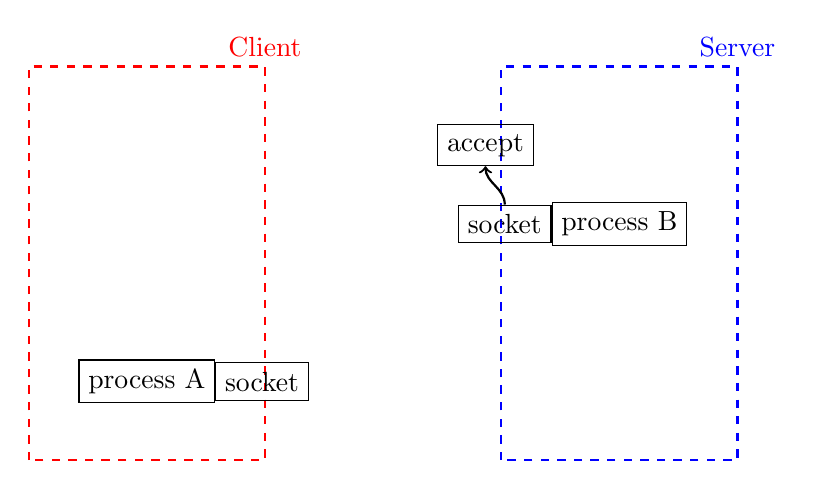
\begin{tikzpicture}
\draw [thick,red,dashed,above] (0,0) rectangle (3,5) node{Client};

%\node [draw,rectangle] (pa3) at(1.5,2){process A3};
\node [draw,rectangle] (pa1) at(1.5,1){process A};
\node [draw,rectangle,right] (cs) at(pa1.east) {socket};

\draw [thick,blue,dashed,above] (6,0) rectangle (9,5)node{Server};
\node [draw,rectangle] (pb1) at(7.5,3){process B};
\node [draw,rectangle,left] (ss) at(pb1.west) {socket};
\node [draw,rectangle] (act) at (5.8,4){accept};
\draw [->,thick] (ss) to[out=90,in=270] (act);
%\draw[thick,->](pa1) to[out=0,in=360] (pa2);
%\draw[thick,->](pa2) to[out=0,in=360] (pa1);
%\draw[thick,->,green](pa3) to[out=0,in=180] (pb1);
%\draw[thick,->,green](pa4) to[out=0,in=270] (pb1);
%\draw[thick,->,green](pb1) to[out=180,in=360] (pa3);
%\draw[thick,->,green](pb1) to[out=270,in=360] (pa4);
\end{tikzpicture}
}
%\end{block}
\end{frame}

\begin{frame}{Socket通信过程 III}
客户端的进程process A创建的socket将服务器的地址和端口传递给connect方法。
%\begin{block}{Socket通信过程}
\center{
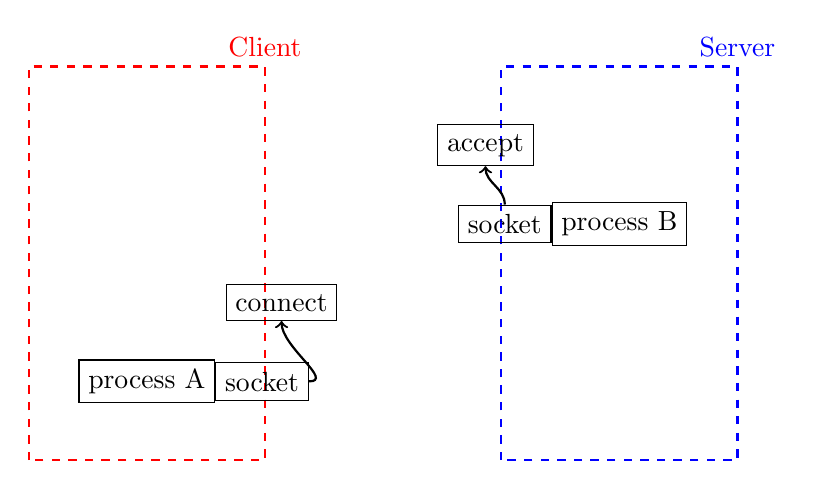
\begin{tikzpicture}
\draw [thick,red,dashed,above] (0,0) rectangle (3,5) node{Client};

%\node [draw,rectangle] (pa3) at(1.5,2){process A3};
\node [draw,rectangle] (pa1) at(1.5,1){process A};
\node [draw,rectangle,right] (cs) at(pa1.east) {socket};
\node [draw,rectangle,right] (conn) at(2.5,2) {connect};
\draw [->,thick] (cs) to[out=0,in=270] (conn);

\draw [thick,blue,dashed,above] (6,0) rectangle (9,5)node{Server};
\node [draw,rectangle] (pb1) at(7.5,3){process B};
\node [draw,rectangle,left] (ss) at(pb1.west) {socket};
\node [draw,rectangle] (act) at (5.8,4){accept};
\draw [->,thick] (ss) to[out=90,in=270] (act);
%\draw[thick,->](pa1) to[out=0,in=360] (pa2);
%\draw[thick,->](pa2) to[out=0,in=360] (pa1);
%\draw[thick,->,green](pa3) to[out=0,in=180] (pb1);
%\draw[thick,->,green](pa4) to[out=0,in=270] (pb1);
%\draw[thick,->,green](pb1) to[out=180,in=360] (pa3);
%\draw[thick,->,green](pb1) to[out=270,in=360] (pa4);
\end{tikzpicture}
}
%\end{block}
\end{frame}

\begin{frame}{Socket通信过程 IV}
客户端与服务端建立连接。然后processA 和B就像操作文件描述符一样可以对socket进行操作了。
%\begin{block}{Socket通信过程}
\center{
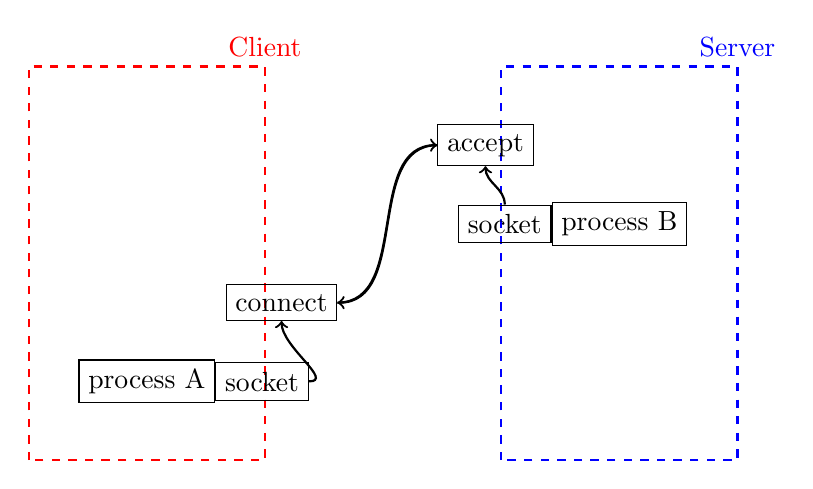
\begin{tikzpicture}
\draw [thick,red,dashed,above] (0,0) rectangle (3,5) node{Client};

%\node [draw,rectangle] (pa3) at(1.5,2){process A3};
\node [draw,rectangle] (pa1) at(1.5,1){process A};
\node [draw,rectangle,right] (cs) at(pa1.east) {socket};
\node [draw,rectangle,right] (conn) at(2.5,2) {connect};
\draw [->,thick] (cs) to[out=0,in=270] (conn);

\draw [thick,blue,dashed,above] (6,0) rectangle (9,5)node{Server};
\node [draw,rectangle] (pb1) at(7.5,3){process B};
\node [draw,rectangle,left] (ss) at(pb1.west) {socket};
\node [draw,rectangle] (act) at (5.8,4){accept};
\draw [->,thick] (ss) to[out=90,in=270] (act);

\draw[->,thick] (conn) to[out=0,in=180] (act);
\draw[->,thick] (act) to[out=180,in=360] (conn);
%\draw[thick,->](pa1) to[out=0,in=360] (pa2);
%\draw[thick,->](pa2) to[out=0,in=360] (pa1);
%\draw[thick,->,green](pa3) to[out=0,in=180] (pb1);
%\draw[thick,->,green](pa4) to[out=0,in=270] (pb1);
%\draw[thick,->,green](pb1) to[out=180,in=360] (pa3);
%\draw[thick,->,green](pb1) to[out=270,in=360] (pa4);
\end{tikzpicture}
}
%\end{block}
\end{frame}

%-----------------------------------------------
\section{Create a Socket}
\begin{frame}
\Huge{\centerline{Create a Socket}}
\end{frame}
\begin{frame}[fragile]{socket系统调用}
socket() creates an endpoint for communication and returns a descriptor.
\begin{block}{原型}
\begin{verbatim}
#include <sys/types.h>         
#include <sys/socket.h>

       int socket(int domain, int type, int protocol);
\end{verbatim}
\end{block}
\end{frame}
\begin{frame}{socket-domain}
     The domain parameter specifies a communications domain within which communication will take place; this selects the protocol family which should be used.  These families are defined in
     the include file <sys/socket.h>.  The domains are as table \ref{skt-dm}.
\begin{table}
\begin{tabular}{ll}
\toprule
\textbf{Name}&\textbf{Purpose}\\
\midrule                                                       
       AF\_UNIX, AF\_LOCAL &  Local communication     \\        
       AF\_INET       &      IPv4 Internet protocols    \\      
       AF\_INET6     &       IPv6 Internet protocols     \\     
 \bottomrule
 \end{tabular}
\caption{Domain of socket}
\label{skt-dm}
\end{table}

\end{frame}
\begin{frame}{socket-type}
     The socket has the indicated type, which specifies the semantics of communication.  Currently defined types\footnote{一部分。} are:
\begin{enumerate}
\item
SOCK\_STREAM
\item   
SOCK\_DGRAM
\end{enumerate}
     A SOCK\_STREAM type provides sequenced, reliable,  connection based byte streams.  An out-of-band data(like urgent mode in tcp) transmission mechanism may be supported.  
     
     A SOCK\_DGRAM socket supports datagrams (connectionless, unreliable messages of a fixed (typically small) maximum length). 
\end{frame}
\begin{frame}{socket-protocol}
The protocol used for communication is usually determined by the socket type and domain. There is normally no choice. The protocol parameter is used where there is a choice. \textcolor{red}{0 }selects the default protocol, which is used in all the examples in our course.
\end{frame}
\begin{frame}{Name a socket}
To make a socket (as created by a call to socket()) available for use by other processes, a server program needs to give the socket a name. 

Thus, AF\_LOCAL sockets are associated with a file system pathname. 

AF\_INET sockets are associated with an IP port number.
\end{frame}
\begin{frame}[fragile]{bind}
\begin{block}{bind原型}
\begin{verbatim}
 #include <sys/types.h>          
 #include <sys/socket.h>

       int bind(int sockfd, const struct sockaddr *addr,
                socklen_t addrlen);
\end{verbatim}
\end{block}
\begin{tikzpicture}
\node (sk) [draw,rectangle] at (0,0) {socket};
\node (des) [draw] at (0,1) {描述符};
\draw [-] (sk) to[out=90,in=270] (des);

\node (add) [draw,rectangle,red] at (3,1) {address};
\draw [-,dashed,thick,above,red] (add) to[out=180,in=360] node{bind}(des);
\end{tikzpicture}

On successful completion, bind returns 0. If it fails, it returns -1 and sets errno .
\end{frame}
\begin{frame}[fragile]{bind-addr}       
       The actual structure passed for the addr argument will depend on the address family.  The sockaddr structure is defined as something like:
\begin{verbatim}
struct sockaddr_in {
  sa_family_t    sin_family; /* address family: AF_INET */
  in_port_t      sin_port;   /* port in network byte order */
  struct in_addr sin_addr;   /* internet address */
};
/* Internet address. */
  struct in_addr {
  uint32_t       s_addr;     /* address in network byte order */
};
\end{verbatim}
The rules used in name binding vary between address families.  Consult the manual entries in Section 7 for detailed information.  For AF\_INET see ip(7), for AF\_INET6 see  ipv6(7),  for  AF\_UNIX  see
       unix(7).
\end{frame}
\begin{frame}[fragile]{create a socket queue}
To accept incoming connections on a socket, a server program must create a queue to store pending requests. It does this using the listen system call.
\begin{block}{listen原型}
\begin{verbatim}
 #include <sys/types.h>  
 #include <sys/socket.h>

       int listen(int sockfd, int backlog);
       \end{verbatim}
\end{block}
The listen function will return 0 on success or -1 on error.
\end{frame}

\begin{frame}[fragile]{accept connection}
Once a server program has created and named a socket, it can wait for connections to be made to the socket by using the accept system call.
\begin{block}{accept原型}
\begin{verbatim}
#include <sys/types.h> 
#include <sys/socket.h>

 int accept(int sockfd, struct sockaddr *addr, 
   socklen_t *addrlen);
\end{verbatim}
\end{block}
The accept system call returns when a client program attempts to connect to the socket specified by the parameter socket. 

The client is the first pending connection from that socket’s queue. 

The accept function creates a new socket to communicate with the client and returns its descriptor. 

The new socket will have the same type as the server listen socket.
\end{frame}
\begin{frame}{accept补充}
If there are no connections pending on the socket’s queue, \textcolor{red}{accept will block }(so that the program won’t continue) until a client does make connection. 

(We can change this behavior by using the O\_NONBLOCK flag on the socket file descriptor, using the fcntl function.)
\end{frame}
\begin{frame}[fragile]{Requesting Connections}
Client programs connect to servers by establishing a connection between an unnamed socket and the server listen socket. We can do this by calling connect.
\begin{block}{connect原型}
\begin{verbatim}
#include <sys/types.h>                
#include <sys/socket.h>
int connect(int sockfd, const struct sockaddr *addr,
                   socklen_t addrlen);
\end{verbatim}
\end{block}
The socket specified by the parameter socket is connected to the server socket specified by the parameter address, which is of length address\_len. The socket must be a valid file descriptor obtained by a call to socket.
If it succeeds, connect returns 0, and -1 is returned on error. 
\end{frame}
\begin{frame}[fragile]{close a socket}
We can terminate a socket connection at the server and client by calling close, just as we would for low-level file descriptors. 
\begin{block}{close原型}
\begin{verbatim}
#include <unistd.h>

     int
     close(int fildes);
\end{verbatim}
\end{block}
\end{frame}
\begin{frame}[fragile]{网络通信-客户端I}
\begin{block}{引入头文件}
\begin{verbatim}
cat client.c 
#include<sys/types.h>
#include<sys/socket.h>
#include<stdio.h>
#include<stdlib.h>
#include<netinet/ip.h>
#include<netinet/in.h>
#include<unistd.h>

\end{verbatim}
\end{block}
\end{frame}

\begin{frame}[fragile]{网络通信-客户端II}
\begin{block}{创建socket连接}
\begin{verbatim}
int main(){
 int sockfd, len, result;
//man 7 ip
 struct sockaddr_in address;
 char ch='C';
 sockfd=socket(AF_INET,SOCK_STREAM,0);
 address.sin_family=AF_INET;
 address.sin_addr.s_addr=inet_addr("127.0.0.1");
 address.sin_port=9980;
 len=sizeof(address);
 result=connect(sockfd,(struct sockaddr *)&address,len);
 if(result==-1){
  perror("oops:client!");
  exit(1);
 }
...
}

\end{verbatim}
\end{block}
\end{frame}
\begin{frame}[fragile]{网络通信-客户端III}
\begin{block}{对socket进行读写操作}
\begin{verbatim}
cat client.c 
int main(){
...	
 write(sockfd,&ch,1);
 read(sockfd,&ch,1);
 printf("char from server is:%c\n",ch);
 close(sockfd);
 exit(0);
}
\end{verbatim}
\end{block}
\end{frame}

\begin{frame}[fragile]{网络通信-服务端I}
\begin{block}{创建一个socket}
\begin{verbatim}
cat server.c
int main(){
 int server_sockfd, client_sockfd;
 int server_len, client_len;
//man 7 ip
 struct sockaddr_in server_address;
 struct sockaddr_in client_address;
 server_sockfd=socket(AF_INET,SOCK_STREAM,0);
...
}

\end{verbatim}
\end{block}
\end{frame}


\begin{frame}[fragile]{网络通信-服务端II}
\begin{block}{bind}
\begin{verbatim}
cat server.c
int main(){
...
server_sockfd=socket(AF_INET,SOCK_STREAM,0);
server_address.sin_family=AF_INET;
server_address.sin_addr.s_addr=inet_addr("127.0.0.1");
server_address.sin_port=9980;
server_len=sizeof(server_address);

bind(server_sockfd,
  (struct sockaddr *)&server_address, 
  server_len);
...
}

\end{verbatim}
\end{block}
\end{frame}



\begin{frame}[fragile]{网络通信-服务端III}
\begin{block}{listen and accept}
\begin{verbatim}
cat server.c
int main(){
...
listen(server_sockfd,5);
while(1){
 char ch;
 printf("serve...\n");
 client_len=sizeof(client_address);
 client_sockfd=accept(server_sockfd,
  (struct sockaddr *)&client_address,
  &client_len);
 read(client_sockfd,&ch,1);
 ch++;
 write(client_sockfd,&ch,1);
 close(client_sockfd);
}
exit(0);
}

\end{verbatim}
\end{block}
\end{frame}

\begin{frame}[fragile]{查看监听的端口号}

\fbox{server\_address.sin\_port=9980;}
当server运行起来时,通过netstat可能会发现本机监听的端口中并没有9980,这是因为通过socket传递的端口号是二进制数字,在各平台上的解析可能不一样。可做以下修改:
\fbox{server\_address.sin\_port=htons(9980);}\footnote{服务器端和客户端程序都要修改。}
\end{frame}
\section{数据报}
\begin{frame}
\Huge{\centerline{数据报}}
\end{frame}
\begin{frame}{数据报}
前面讲解的都是基于连接的通信方式(TCP)。
当有些通信对数据的丢失不敏感或要求数据的质量不高的时候,可以考虑使用数据报来传递数据,对应到传输协议就是UDP协议。

编写udp服务程序,与tcp最明显的不同之处在于:需要使用两个数据报专用的系统调用sendto和recvfrom来代替read和write调用。
\end{frame}

\begin{frame}{数据报通信过程}

%\begin{block}{Socket通信过程}
\center{
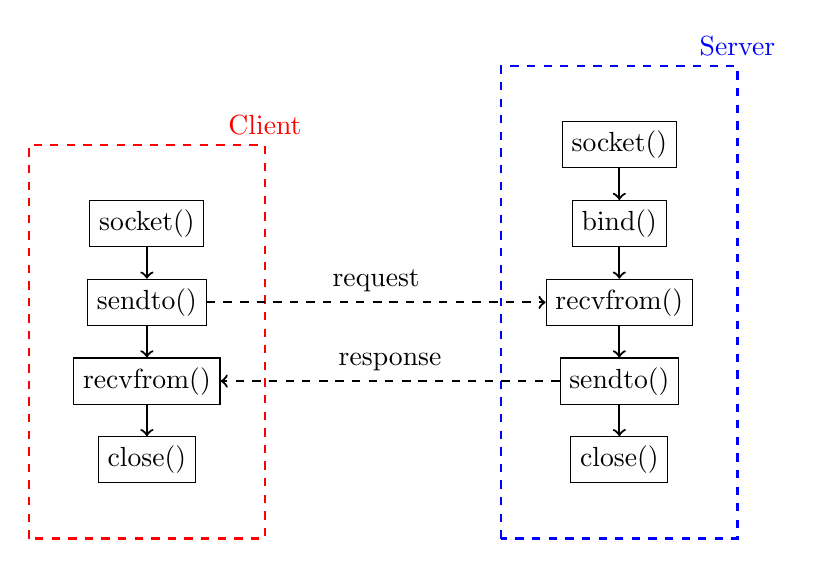
\begin{tikzpicture}
\draw [thick,red,dashed,above] (0,0) rectangle (3,5) node{Client};
\node [draw,rectangle] (skt) at(1.5,4){socket()};
\node [draw,rectangle] (sd) at(1.5,3){sendto()};
\node [draw,rectangle] (rec) at(1.5,2){recvfrom()};
\node [draw,rectangle] (clo) at(1.5,1){close()};
\draw [thick,blue,dashed,above] (6,0) rectangle (9,6)node{Server};
\node [draw,rectangle] (sskt) at(7.5,5){socket()};
\node [draw,rectangle] (sbd) at(7.5,4){bind()};
\node [draw,rectangle] (srec) at(7.5,3){recvfrom()};
\node [draw,rectangle] (ssd) at(7.5,2){sendto()};
\node [draw,rectangle] (sclo) at(7.5,1){close()};
\draw [->,thick] (skt) -- (sd);
\draw [->,thick] (sd) -- (rec);
\draw [->,thick] (rec) -- (clo);

\draw [->,thick] (sskt) -- (sbd);
\draw [->,thick] (sbd) -- (srec);
\draw [->,thick] (srec) -- (ssd);
\draw [->,thick] (ssd) -- (sclo);
\draw[->,dashed,thick,above] (sd) to[out=0,in=180] node{request} (srec);
\draw[->,dashed,thick,above] (ssd) to[out=180,in=0] node{response} (rec);
%\draw[thick,->](pa1) to[out=0,in=360] (pa2);
%\draw[thick,->](pa2) to[out=0,in=360] (pa1);
%\draw[thick,->,green](pa3) to[out=0,in=180] (pb1);
%\draw[thick,->,green](pa4) to[out=0,in=270] (pb1);
%\draw[thick,->,green](pb1) to[out=180,in=360] (pa3);
%\draw[thick,->,green](pb1) to[out=270,in=360] (pa4);
\end{tikzpicture}
}
%\end{block}
\end{frame}



\begin{frame}[fragile]{数据报例子-客户端}
\begin{block}{clientUDP.c}
\begin{verbatim}
sockfd=socket(AF_INET,SOCK_DGRAM,0);
address.sin_family=AF_INET;
address.sin_addr.s_addr=inet_addr("127.0.0.1");
address.sin_port=htons(9980);
len=sizeof(address);

printf("input a char:");
buf=getchar();
int rz = sendto(sockfd,&buf,1,0,
  (struct sockaddr *)&address,len);
\end{verbatim}
\end{block}
\end{frame}

\begin{frame}[fragile]{数据报例子-服务端}
\begin{block}{serverUDP.c}
\begin{verbatim}
server_sockfd=socket(AF_INET,SOCK_DGRAM,0);
 server_address.sin_family=AF_INET;
 server_address.sin_addr.s_addr=inet_addr("127.0.0.1");
 server_address.sin_port=htons(9980);
 server_len=sizeof(server_address);
 bind(server_sockfd,
   (struct sockaddr *)&server_address,server_len);

while(1){
  char ch;
  printf("UDP serve...\n");
  recvfrom(server_sockfd,buf,1,0,
    (struct sockaddr *)&server_address,&server_len);
  printf("the client sent:%s",buf);
}

\end{verbatim}
\end{block}
\end{frame}
%------------------------------------------------
%------------------------------------------------
%\section{Signal}
%\begin{frame}
%\Huge{\centerline{Signal}}
%\end{frame}
%------------------------------------------------
%------------------------------------------------
\begin{frame}{作业}
编写一个socket程序,要求:
\begin{enumerate}
\item
使用TCP协议实现
\item
客户端可以和服务器端进行通信
\item
当用户输入end时,本客户端退出结束
\item
进阶要求:
\begin{enumerate}
\item
多个客户端可以同时分别和服务端通信
\item
实现一个类似聊天室的功能
\end{enumerate}

\end{enumerate}
\end{frame}

\begin{frame}
\Huge{\centerline{The End}}
\end{frame}



\section{Appendix}
\begin{frame}
\Huge{\centerline{Appendix}}
\end{frame}
%----------------------------------------------------------------------------------------
\begin{frame}{本课程相关资源下载}
\begin{enumerate}
\item
ppt

\url{https://github.com/gmsft/ppt/tree/master/linux}
\item
实验指导书

\url{https://github.com/gmsft/ppt/tree/master/book/linux}
\end{enumerate}
\end{frame}
\begin{frame}
\frametitle{about man page}
The manual is generally split into eight numbered sections, organized as follows (on Research Unix, BSD, macOS and Linux):
\begin{table}
\begin{tabular}{ll}
\toprule
\textbf{section} & \textbf{description} \\
\midrule
1 & General commands\\
2 & System calls\\
3 & Library function(C standard library)\\
4 & Special files(devices) and drivers\\
5 & File formats and conventions\\
6 & Games and screensavers\\
7 & Miscellanea\\
8 & System administration commands and daemons\\  
\bottomrule
\end{tabular}
\caption{man page}
\end{table}

在终端中运行man read 与 man 2 read ,观察其输出的区别。
\end{frame}

\end{document} 
